% =====================================================================
%  Research Paper — Media-Search
%  Single-column dissertation-style format (matching 6839387 reference)
%  Title: Two-Stage CLIP Re-Ranking with VLM-Augmented Hybrid Search
%         for Scalable Personal Image Retrieval
%  Author: Aryan Nilesh Marthak (220170111007)
% =====================================================================

\documentclass[12pt,a4paper,oneside]{report}

% ------------------------------------------------------------------ %
%  Packages                                                           %
% ------------------------------------------------------------------ %
\usepackage[T1]{fontenc}
\usepackage[utf8]{inputenc}
\usepackage{amsmath,amssymb}
\usepackage{mathptmx}           % Times New Roman compatible
\usepackage[
  left=1in, right=1in,
  top=1in,  bottom=1in
]{geometry}
\usepackage{setspace}
\usepackage{graphicx}
\graphicspath{{../Report/}{../images/diagrams/}{../Report/screenshots/}}
\usepackage{fancyhdr}
\usepackage{titlesec}
\usepackage{parskip}
\usepackage{enumitem}
\usepackage{array}
\usepackage{longtable}
\usepackage{booktabs}
\usepackage{tabularx}
\usepackage{caption}
\usepackage{float}
\usepackage{url}
\usepackage{xurl}
\usepackage{hyperref}
\usepackage{xcolor}
\usepackage{listings}

% ------------------------------------------------------------------ %
%  Hyperref setup                                                     %
% ------------------------------------------------------------------ %
\hypersetup{
  colorlinks = true,
  linkcolor  = black,
  citecolor  = black,
  urlcolor   = black,
  pdftitle   = {Two-Stage CLIP Re-Ranking with VLM-Augmented Hybrid
                Search for Scalable Personal Image Retrieval},
  pdfauthor  = {Aryan Nilesh Marthak}
}

% ------------------------------------------------------------------ %
%  Global spacing                                                     %
% ------------------------------------------------------------------ %
\onehalfspacing
\setlength{\parindent}{0pt}
\setlength{\parskip}{0.6em}
\setlength{\emergencystretch}{4em}
\hbadness=10000
\tolerance=9999
\hyphenpenalty=10000
\exhyphenpenalty=10000

% ------------------------------------------------------------------ %
%  Page styles                                                        %
% ------------------------------------------------------------------ %
\setlength{\headheight}{14pt}

\fancypagestyle{mainpages}{%
  \fancyhf{}%
  \fancyfoot[L]{\small\thepage}%
  \fancyfoot[R]{\small 220170111007}%
  \renewcommand{\headrulewidth}{0pt}%
  \renewcommand{\footrulewidth}{0pt}%
}

\fancypagestyle{plain}{%
  \fancyhf{}%
  \fancyfoot[L]{\small\thepage}%
  \fancyfoot[R]{\small 220170111007}%
  \renewcommand{\headrulewidth}{0pt}%
  \renewcommand{\footrulewidth}{0pt}%
}

\pagestyle{mainpages}

% ------------------------------------------------------------------ %
%  Chapter / section formatting (matching 6839387 style)              %
% ------------------------------------------------------------------ %
\titleformat{\chapter}[display]
  {\normalfont\bfseries\centering}
  {\fontsize{12}{14.4}\selectfont CHAPTER \thechapter}{0pt}
  {\fontsize{14}{16.8}\selectfont\MakeUppercase}
\titlespacing*{\chapter}{0pt}{-10pt}{20pt}

\titleformat{name=\chapter,numberless}[display]
  {\normalfont\bfseries\centering}
  {}{0pt}
  {\fontsize{14}{16.8}\selectfont\MakeUppercase}

\titleformat{\section}
  {\normalfont\fontsize{12}{14.4}\selectfont\bfseries\itshape}
  {\thesection}{1em}{}

\titleformat{\subsection}
  {\normalfont\fontsize{12}{14.4}\selectfont\bfseries}
  {\thesubsection}{1em}{}

\titleformat{\subsubsection}
  {\normalfont\normalsize\itshape}
  {\thesubsubsection}{1em}{}

\renewcommand{\chaptermark}[1]{\markboth{#1}{}}

% ------------------------------------------------------------------ %
%  Listings                                                           %
% ------------------------------------------------------------------ %
\definecolor{codegray}{rgb}{0.95,0.95,0.95}

\lstset{
  backgroundcolor  = \color{codegray},
  basicstyle       = \ttfamily\small,
  breaklines       = true,
  frame            = single,
  numbers          = none,
  tabsize          = 2,
}

% ====================================================================
%  DOCUMENT START
% ====================================================================
\begin{document}
\pagenumbering{arabic}

% ====================================================================
%  TITLE PAGE
% ====================================================================
\begin{titlepage}
\thispagestyle{empty}
\begin{center}
\begin{singlespace}

\vspace*{3cm}

{\LARGE\textbf{Two-Stage CLIP Re-Ranking with\\[6pt]
VLM-Augmented Hybrid Search for\\[6pt]
Scalable Personal Image Retrieval}}

\vspace{2.5cm}

{\large Aryan Nilesh Marthak}\\[8pt]
Enrolment No.: 220170111007\\[8pt]
Department of Electronics \& Communication Engineering\\[8pt]
Vishwakarma Government Engineering College\\[8pt]
Gujarat Technological University, Ahmedabad

\vspace{2.5cm}

A Research Paper\\[8pt]
submitted in partial fulfilment of the requirements for the degree of\\[8pt]
\textbf{Bachelor of Engineering}\\[8pt]
in\\[8pt]
\textbf{Electronics \& Communication Engineering}

\vspace{2cm}

April 2026

\end{singlespace}
\end{center}
\end{titlepage}

% ====================================================================
%  ABSTRACT
% ====================================================================
\clearpage
\chapter*{Abstract}
\addcontentsline{toc}{chapter}{Abstract}

Personal image collections are growing rapidly, yet retrieval methods remain limited to filename matching and manual tagging. This paper presents Media-Search, a self-hosted, AI-powered image retrieval system that combines a two-stage CLIP-based search pipeline with a hybrid BM25-CLIP deep search over Vision-Language Model (VLM) generated descriptions.

The first stage uses a frozen CLIP ViT-L/14 encoder for global recall from a Qdrant vector database. The second stage re-ranks candidates using local crop embeddings, generating five crops per image (one centre crop and four quadrant crops) to capture spatially localised objects that global embeddings tend to miss. A complementary deep search mode fuses BM25 keyword scores over SmolVLM-generated image descriptions with CLIP semantic similarity. The system also integrates DeepFace-based face detection with DBSCAN clustering for person-based retrieval.

Evaluation on a 100-image Flickr8k subset with 499 queries demonstrates a mean Average Precision (mAP) of 0.9177 for CLIP search with local re-ranking, a Recall@20 of 0.9790, and a query success rate of 95.8\%, with median end-to-end latency under 150 ms leveraging an NVIDIA RTX 3050 GPU. The hybrid BM25-CLIP mode achieves an mAP of 0.7169, performing best on attribute-specific queries that benefit from the explicit textual detail in VLM descriptions. The two modes are shown to be complementary rather than competing, suited to different query types.

\textbf{Categories:} cs.CV (Computer Vision), cs.IR (Information Retrieval)

\textbf{Keywords:} CLIP, image retrieval, vision-language models, BM25, hybrid search, face clustering, DBSCAN, vector database, local re-ranking, self-hosted

% ====================================================================
%  TABLE OF CONTENTS
% ====================================================================
\clearpage
\tableofcontents

% ====================================================================
%  CHAPTER 1 — INTRODUCTION
% ====================================================================
\chapter{Introduction}

\section{Background}

The proliferation of personal photography devices has led to users accumulating thousands of photographs annually, encompassing events, documents, and general daily life. Locating a specific image within such vast collections remains a significant retrieval challenge. Users are typically forced to manually navigate extensive galleries or rely on temporal metadata, which has limited efficacy when the exact capture date is unknown.

Commercial cloud services address this using proprietary machine learning models; however, these solutions are closed-source, necessitate the transfer of personal data to third-party servers, and provide limited transparency into their retrieval algorithms. For privacy-conscious users and organisations requiring on-premise solutions, a substantial gap exists in available retrieval platforms.

A fundamental technical limitation of prevailing retrieval architectures is their reliance on encoding an entire image into a single global embedding vector. While effective for capturing holistic scene semantics, global pooling mechanisms frequently attenuate localized, fine-grained visual priors---such as small objects, specific facial features, or background text. Consequently, queries targeting localized regions (e.g., a small object within a cluttered scene) often yield high false-positive rates, as the global embedding prioritizes dominant background elements while neglecting independent spatial features.

Content-based image retrieval (CBIR) architectures were initially developed to address the constraints of metadata-dependent search by indexing images based on intrinsic visual properties. Early iterations utilized hand-crafted heuristics, including colour histograms, edge density maps, and texture descriptors. Despite providing foundational improvements, these primitive descriptors failed to sufficiently bridge the semantic gap between low-level pixel matrices and high-level conceptual queries.

The advent of deep convolutional neural networks (CNNs), pre-trained on large-scale annotated datasets, significantly mitigated this semantic disconnect. Latent vector representations extracted from CNN architectures correlate robustly with human perception. Nonetheless, traditional CNN retrieval paradigms remained unimodal, fundamentally requiring visual query inputs and failing to support zero-shot natural language querying.

Recent advancements in contrastive vision-language pre-training, notably the CLIP (Contrastive Language-Image Pre-training) architecture [1], have revolutionized this paradigm. By aligning image and text representations within a shared multi-modal embedding space, CLIP facilitates highly accurate zero-shot retrieval utilizing unconstrained natural language vectors. This enables robust semantic matching without dependency on antecedent hierarchical categorizations or rigid folder taxonomies.

\section{Problem Statement}

Given an arbitrarily large personal image collection with no manual labels and variable quality, the problem is to build a system that returns a ranked list of relevant images for a free-text query, with calibrated confidence scores, in under 5 seconds on commodity hardware.

The operating constraints are highly demanding:
\begin{itemize}[leftmargin=*]
  \item Images in personal collections typically lack manual annotations or metadata tagging.
  \item Image quality exhibits significant variance, ranging from high-resolution photographs to low-quality captures with noise or motion blur.
  \item Retrieval latency must be minimal, as interactive search delays critically degrade the user experience.
  \item The system must operate efficiently on consumer-grade graphics hardware (e.g., an NVIDIA RTX 3050 GPU) without reliance on cloud GPU clusters.
  \item Data processing must remain local, as transferring personal visual data to third-party servers raises significant privacy and security concerns.
\end{itemize}

More specifically, the problem decomposes into four sub-problems: (a) encoding both images and text queries into a shared semantic embedding space and performing efficient approximate nearest-neighbour search over that space; (b) generating rich textual descriptions of uploaded images using a vision-language model to enable complementary keyword-based search; (c) detecting faces within images, computing face embeddings, and automatically grouping them by identity using unsupervised clustering; (d) integrating all AI components into a secure, multi-user web application with authentication and real-time processing progress updates.

\section{Research Questions}

\begin{itemize}[leftmargin=*]
  \item \textbf{RQ1}: Does local crop re-ranking significantly improve retrieval precision compared to global-only CLIP retrieval?
  \item \textbf{RQ2}: Does a BM25 + CLIP hybrid approach on VLM descriptions outperform either modality used alone?
  \item \textbf{RQ3}: How does the choice of score fusion weights affect the tradeoff between precision and query latency?
  \item \textbf{RQ4}: Can DBSCAN-based face clustering provide usable person-based search in uncurated personal collections?
\end{itemize}

\section{Contributions}

This paper makes the following contributions:

\begin{enumerate}[leftmargin=*]
  \item A \textbf{two-stage CLIP retrieval pipeline} combining ViT-L/14 global recall with local crop re-ranking (five crops per image), improving precision for queries targeting localised objects.
  \item A \textbf{hybrid deep search mode} fusing BM25 keyword matching over VLM-generated image descriptions with CLIP semantic similarity, covering both exact-keyword and paraphrase queries.
  \item \textbf{Automated face detection and clustering} using DeepFace (RetinaFace + ArcFace) with DBSCAN, enabling person-based retrieval without manual labelling.
  \item A \textbf{production-quality system} deployed as a multi-user web application (FastAPI, React, Qdrant, PostgreSQL) with JWT authentication and real-time SSE processing feedback.
  \item \textbf{Quantitative evaluation} on a standard academic dataset (Flickr8k) with 499 queries, providing reproducible performance benchmarks.
\end{enumerate}

\section{Paper Organisation}

The remainder of this paper is organised as follows. Chapter 2 surveys related work across vision-language pre-training, two-stage retrieval, hybrid search, face clustering, and vector databases. Chapter 3 describes the system architecture and search pipeline methodology. Chapter 4 details the experimental setup, including the dataset, evaluation metrics, and baselines. Chapter 5 presents the results and analysis. Chapter 6 concludes with a summary of contributions, limitations, and directions for future work.


% ====================================================================
%  CHAPTER 2 — LITERATURE REVIEW
% ====================================================================
\chapter{Literature Review}

\section{Overview}

This chapter surveys the principal bodies of research that directly influenced the design of the Media-Search system: vision-language pre-training for semantic image-text alignment, two-stage cascade retrieval for improved precision, vision-language models for image captioning, face detection and clustering for identity-based retrieval, hybrid keyword-semantic search, and vector databases for approximate nearest-neighbour search. Each section identifies the key contributions and their limitations, building towards the gaps that this project addresses.

\section{Vision-Language Pre-Training and CLIP}

CLIP (Contrastive Language-Image Pre-training), introduced by Radford et al.\ [1] at OpenAI in 2021, trains a vision encoder and text encoder jointly on approximately 400 million image-text pairs collected from the internet. The training uses a contrastive learning objective that maximises the cosine similarity between paired image and text embeddings while minimising it for unpaired combinations. The result is a shared embedding space in which semantically related images and texts are geometrically close, regardless of their surface-level visual or lexical differences.

CLIP's most significant contribution to practical image retrieval is the ability to embed both a natural language query and an image collection in the same metric space, enabling direct text-to-image similarity search. Unlike earlier cross-modal retrieval systems that required separate retrieval and re-ranking stages in different feature spaces, CLIP's unified embedding space makes the retrieval pipeline conceptually and computationally straightforward: encode the query with the text encoder, compute cosine similarities against the image embedding database, and return the top-$k$ results.

The ViT-L/14 variant of CLIP, which uses a Vision Transformer (ViT) [2] with patch size 14 and a large architecture, achieves the strongest zero-shot retrieval performance among the publicly available CLIP variants. It produces 768-dimensional embeddings that offer significantly richer semantic representations than the smaller ViT-B/32 (512-dimensional). This project uses ViT-L/14 via the OpenCLIP [3] library, which provides the pre-trained weights and a clean Python API.

Several works following CLIP explored improved training objectives. SigLIP [4] (Sigmoid Loss for Language-Image Pre-training) replaced CLIP's softmax-normalised contrastive loss with a pairwise sigmoid loss that does not require synchronisation across the full training batch, improving training stability and yielding better performance at the same model size.

One persistent limitation is worth noting: CLIP encodes an entire image into a single vector. Spatial information, such as where objects are located in the frame, gets compressed away. This is likely a problem for queries targeting specific objects within a larger scene. A query for ``red umbrella'' might retrieve images dominated by red colour without any umbrella present.

\section{Two-Stage Retrieval and Local Re-Ranking}

While the global CLIP embedding of an image captures its overall semantic content, it may fall short when the query refers to a localised object within a complex scene. For example, a query for ``red umbrella'' may retrieve an image in which the umbrella is a minor element in a corner if the global embedding is dominated by the more visually prominent foreground subject.

Two-stage retrieval pipeline designs address this limitation. The first stage performs efficient approximate nearest-neighbour search over global embeddings to retrieve a set of candidates. The second, re-ranking stage applies a more detailed computation to these candidates to produce the final ranked list. This cascade paradigm is well established in the information retrieval literature [5]: broad recall in the first stage is refined by precise ranking in the second.

Media-Search adapts this paradigm by computing CLIP embeddings for multiple image crops in the re-ranking stage, rather than relying on traditional local feature detectors such as SIFT or SuperPoint. The rationale is that the object of interest is likely to be well-represented in at least one crop of the candidate image, even if it is not the dominant subject at the global scale.

\section{Vision-Language Models for Image Captioning}

Beyond embedding-based retrieval, rich natural language descriptions of images provide an alternative search surface that can be indexed with keyword matching. The SmolVLM model [6] by HuggingFace is a compact but capable vision-language model that generates detailed natural language descriptions of images. Unlike CLIP, which projects images and text into a shared embedding space, SmolVLM is a generative model that produces free-form text descriptions of arbitrary length and detail.

The use of a vision-language model for generating search-optimised image descriptions builds on a body of work in cross-modal retrieval that combines image captioning with text-based indexing. Modern open VLMs such as SmolVLM produce open-ended natural language descriptions that are richer and more informative for search purposes than the template-based or structured scene-graph captions used in earlier approaches.

However, generative models are not infallible. They occasionally hallucinate details that seem plausible but are factually absent from the image. This is a known issue across all VLM architectures and directly affects the precision of any downstream text-based search.

\section{Hybrid Keyword-Semantic Search}

While dense vector retrieval excels at semantic similarity, it can underperform on queries that require exact keyword matching. BM25 (Best Match 25) [7], introduced by Robertson et al., is a well-established TF-IDF-based ranking function that scores documents by term frequency, inverse document frequency, and document length normalisation.

Hybrid search systems that combine BM25 keyword scores with dense embedding similarity scores have been shown to outperform either approach in isolation across a range of retrieval benchmarks [8]. The key insight is that BM25 and dense retrieval are complementary: BM25 is strong on queries with specific rare keywords, while dense retrieval handles paraphrase and synonym queries better. Their combination is therefore more robust than either alone.

\section{Face Detection and Clustering}

Face detection is a well-studied problem in computer vision. Media-Search uses DeepFace [9], a lightweight Python library that wraps several state-of-the-art face detection and recognition models behind a unified API. The library provides both face localisation (bounding boxes) and face representation (computing a numerical embedding for each detected face). ArcFace, the recognition model used for face embedding, is trained with an additive angular margin loss that produces highly discriminative embeddings in a hyperspherical space.

DBSCAN (Density-Based Spatial Clustering of Applications with Noise) [10], introduced by Ester et al., is a parameter-free alternative to k-means that groups embeddings by local density, automatically determining the number of clusters and labelling outlier embeddings as noise. DBSCAN is particularly well-suited to face clustering because it handles variable-size clusters naturally, explicitly models unclustered faces, and requires only two hyperparameters: the neighbourhood radius $\varepsilon$ and the minimum cluster size.

\section{Vector Databases}

Exact nearest-neighbour search is computationally intractable for high-dimensional embeddings at scale. ANN algorithms trade a small amount of recall for dramatically reduced search latency through data structures such as HNSW (Hierarchical Navigable Small World graphs) [11].

Qdrant [12] is a vector similarity database built on the HNSW algorithm that provides fast ANN search with rich filtering capabilities. A feature that is particularly valuable for multi-user systems is Qdrant's payload filtering: each stored vector can carry an arbitrary JSON payload, and search queries can include a filter that restricts results to vectors matching specific payload fields. This mechanism is used in Media-Search to enforce per-user data isolation without maintaining separate collections per user.

\section{Gaps in Current Work}

From the literature reviewed, several gaps stand out:

\begin{enumerate}[leftmargin=*]
  \item No published work (that we have found) combines CLIP local crop re-ranking with BM25/VLM hybrid scoring in a single integrated system.
  \item Personal image retrieval under no-label, mixed-quality conditions is underexplored. Most evaluations assume clean, curated datasets.
  \item Face clustering is usually treated as a standalone problem rather than integrated into a unified retrieval pipeline.
  \item Existing open-source image search tools lack the combination of CLIP semantic search, VLM descriptions, face clustering, and multi-user support.
\end{enumerate}

This project attempts to address all four gaps.


% ====================================================================
%  CHAPTER 3 — SYSTEM ARCHITECTURE AND METHODOLOGY
% ====================================================================
\chapter{System Architecture and Methodology}

\section{System Overview}

Media-Search is a three-tier web application composed of a React 18 SPA frontend, a FastAPI backend organised into four routers (\texttt{auth}, \texttt{images}, \texttt{search}, \texttt{faces}), and supporting data services (Qdrant, PostgreSQL, Redis). Three AI service modules encapsulate all model logic: \texttt{embedding\_service} (CLIP), \texttt{vlm\_service} (SmolVLM), and \texttt{face\_service} (DeepFace). Figure~\ref{fig:arch} illustrates the high-level architecture.

\begin{figure}[H]
\centering
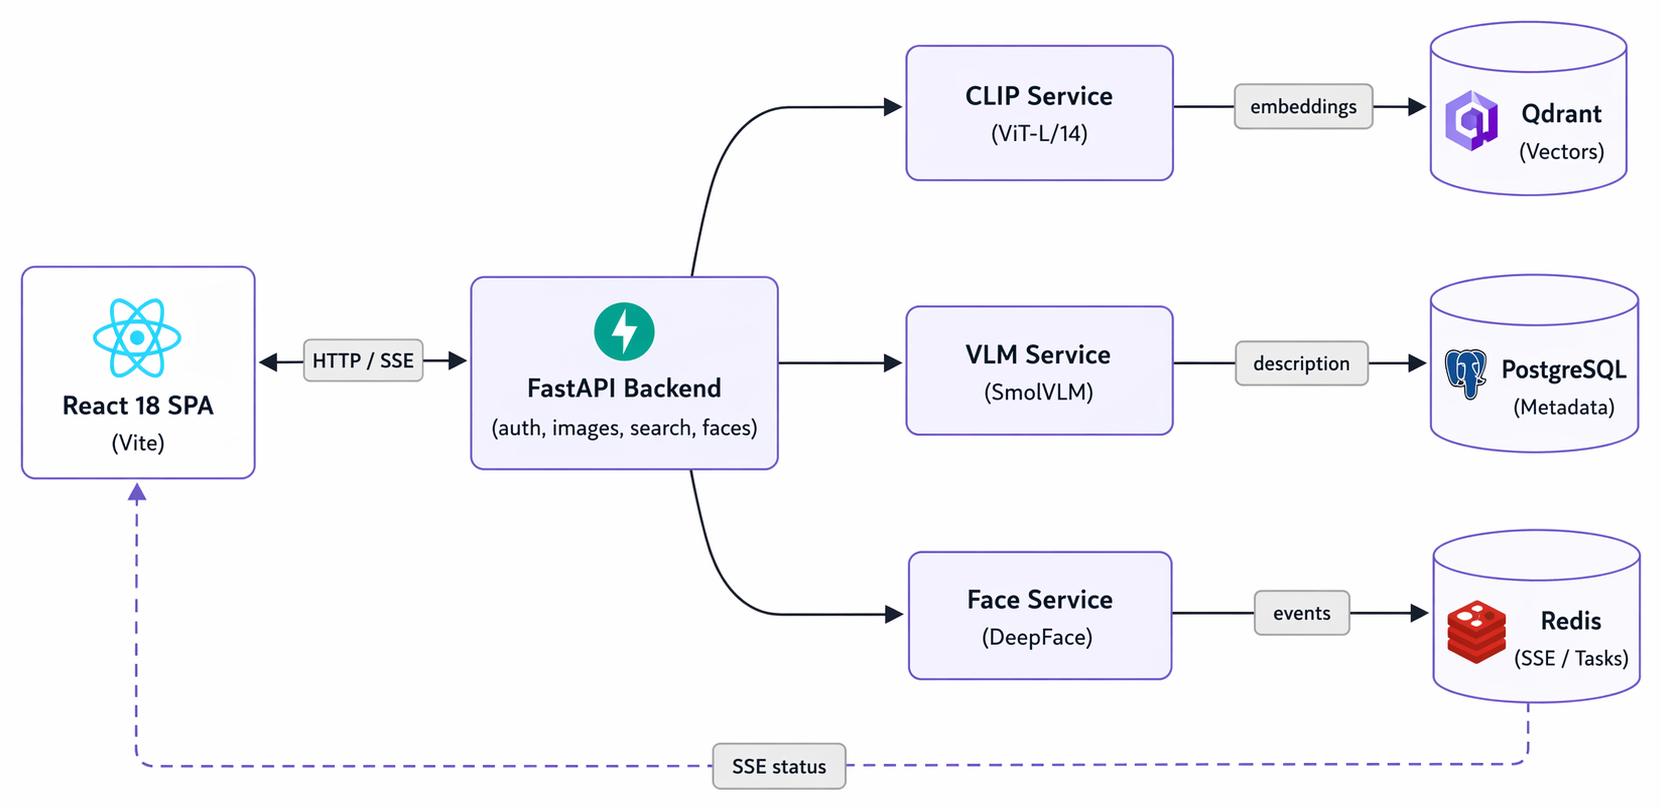
\includegraphics[width=\linewidth]{1d.png}
\caption{High-level system architecture of the Media-Search system}
\label{fig:arch}
\end{figure}

The React SPA communicates with the FastAPI backend exclusively over HTTP (REST + SSE). All routes require a valid JWT token in the \texttt{Authorization: Bearer} header, except \texttt{/auth/register} and \texttt{/auth/login}. Three AI service modules encapsulate all model logic. Their outputs flow to the appropriate data stores: CLIP embeddings to Qdrant, VLM descriptions to PostgreSQL, and face thumbnails to the local filesystem. Redis is used as an event bus for SSE status messages and as a lightweight task coordination layer.

\section{Image Processing Pipeline}

On upload, each image passes through three processing stages:

\begin{enumerate}[leftmargin=*]
  \item \textbf{CLIP Embedding:} The image is encoded by ViT-L/14 into a 768-dimensional vector, which is normalised and stored in Qdrant with the owner's \texttt{user\_id} as a payload field. Image metadata (filename, size, MIME type, upload timestamp, storage path) is stored in PostgreSQL.
  \item \textbf{VLM Description Generation:} SmolVLM [6] generates a detailed natural language description of the image. This runs asynchronously as a background task after the upload response has been returned to the client. The description is stored in PostgreSQL alongside the image metadata.
  \item \textbf{Face Detection and Clustering:} DeepFace detects all faces in the image, computes 512-dimensional ArcFace embeddings for each detected face, and stores face thumbnails on the filesystem. DBSCAN ($\varepsilon = 0.5$, $\text{min\_samples} = 3$) clusters faces by identity. Users can assign names to discovered clusters.
\end{enumerate}

Real-time processing status is streamed to the browser via Server-Sent Events (SSE) through a Redis pub/sub channel keyed by image ID. A pixel-art badge in the frontend shows the current pipeline stage for each image (embedding complete, VLM processing, face detection done).

\section{Search Pipeline}

The system supports three progressively deeper search modes, each more computationally intensive than the last.

\subsection{Mode 1: Global CLIP Search}

The query string is first passed through automatic spell-correction using a BK-tree based corrector, then encoded by the CLIP text encoder to produce a 768-dimensional query embedding $\mathbf{q}$. Qdrant is queried with $\mathbf{q}$ using cosine similarity, filtered to documents owned by the current user. The top-$k$ results (default $k = 20$) are returned ranked by global cosine similarity score.

This mode is the fastest (median 65 ms end-to-end) and handles broad semantic queries effectively. However, it may miss images where the queried object is a small element within a larger scene.

\subsection{Mode 2: CLIP Search with Local Re-Ranking}

Steps are identical to Mode 1 for candidate retrieval. After the candidate set is retrieved, each candidate undergoes local crop analysis:

\begin{enumerate}[leftmargin=*]
  \item Five crops are generated on-the-fly from each candidate image: one centre crop (60\% of the shorter dimension) and four quadrant crops (top-left, top-right, bottom-left, bottom-right, each 50\% of each dimension).
  \item Each crop is encoded by the CLIP image encoder to produce five local embeddings.
  \item The local score $S_{\text{local}}$ for a candidate is the maximum cosine similarity between $\mathbf{q}$ and any of its five crop embeddings.
  \item The final score combines global and local signals:
\end{enumerate}

\begin{equation}
  S_{\text{final}} = 0.6 \times S_{\text{global}} + 0.4 \times S_{\text{local}}
  \label{eq:rerank}
\end{equation}

The 60/40 weighting was determined empirically. The global score anchors the result in overall semantic relevance, while the local score boosts candidates where the queried object is clearly visible in at least one region.

\subsection{Mode 3: Deep Hybrid Search (BM25 + CLIP)}

For attribute-specific queries where exact keywords matter (e.g., ``person wearing a striped blue shirt''), a hybrid approach combines keyword and semantic scoring:

\begin{enumerate}[leftmargin=*]
  \item A BM25 index is built at query time over all VLM-generated descriptions belonging to the current user.
  \item The query is scored against the BM25 index; scores are normalised to $[0, 1]$ by dividing by the maximum score.
  \item The query is also used for CLIP semantic scoring (Mode 1).
  \item Results from BM25 and CLIP are merged (union of candidate sets).
  \item The final hybrid score is:
\end{enumerate}

\begin{equation}
  S_{\text{hybrid}} = 0.7 \times S_{\text{BM25}}^{(\text{norm})} + 0.3 \times S_{\text{CLIP}}
  \label{eq:hybrid}
\end{equation}

BM25 receives the majority weight because VLM descriptions tend to be rich in specific keywords (colours, object names, clothing descriptions) that strongly discriminate between images. CLIP's 30\% contribution ensures that semantically relevant images are not excluded if the VLM happened to use different phrasing.

\section{Score Calibration}

Raw similarity scores from CLIP are not naturally calibrated as probabilities. To produce meaningful confidence scores, raw scores are passed through a temperature-scaled sigmoid function:

\begin{equation}
  \text{score}_{\text{cal}} = \sigma(\tau \cdot S)
  \label{eq:calibration}
\end{equation}

where $\tau$ is the temperature parameter. Higher temperatures ($\tau \in [25, 35]$) produce stricter filtering with fewer but more confident results. Lower temperatures ($\tau \in [15, 18]$) are more lenient, returning more results at the cost of some noise.

\section{Face Search}

When a user searches by person name, the system retrieves the corresponding DBSCAN cluster label, then returns all images containing faces assigned to that cluster. Users can manually assign name labels to discovered clusters, merge clusters that correspond to the same person, and relabel them as needed.

\section{Technology Stack}

Table~\ref{tab:tech} summarises the technology choices and their rationale.

\begin{table}[H]
\centering\small
\caption{Technology Choices and Rationale}
\label{tab:tech}
\renewcommand{\arraystretch}{1.4}
\begin{tabular}{|p{2.8cm}|p{3.2cm}|p{7.2cm}|}
\hline
\textbf{Component} & \textbf{Technology} & \textbf{Rationale} \\
\hline
Web Framework & FastAPI & Async-native, auto-generates OpenAPI docs, Pydantic validation. \\
\hline
Database ORM & SQLAlchemy 2.0 & Async ORM with asyncpg driver for non-blocking PostgreSQL access. \\
\hline
Relational DB & PostgreSQL & ACID compliance, JSONB support, integrates with asyncpg. \\
\hline
Vector DB & Qdrant & HNSW-based ANN search with payload filtering for per-user isolation. \\
\hline
CLIP Model & OpenCLIP ViT-L/14 & High-performance open-source zero-shot retrieval; 768-dimensional embeddings. \\
\hline
VLM & SmolVLM & Compact generative VLM; produces detailed descriptions without GPU. \\
\hline
Face Pipeline & DeepFace & Wraps RetinaFace (detection) and ArcFace (recognition) in one API. \\
\hline
Clustering & DBSCAN & Auto-determines cluster count; labels noise faces explicitly. \\
\hline
Frontend & React 18 + Vite & Fast SPA toolchain with hooks for auth context, SSE, and routing. \\
\hline
Containerisation & Docker Compose & Single command starts all supporting services reproducibly. \\
\hline
\end{tabular}
\end{table}


% ====================================================================
%  CHAPTER 4 — EXPERIMENTAL SETUP
% ====================================================================
\chapter{Experimental Setup}

\section{Dataset}

To rigorously evaluate the system's retrieval performance, a subset of the standard academic Flickr8k dataset [13] was utilised. A test library of 100 images was randomly sampled from the dataset, ensuring a diverse range of subjects including landscapes, portraits, animals, and complex indoor/outdoor scenes. The dataset's pre-annotated captions (five per image, totalling 499 unique evaluation queries after removing one duplicate) were used as the ground-truth matches for querying.

All 100 images were ingested into the Media-Search system through the standard upload pipeline: each image was embedded by CLIP ViT-L/14, described by SmolVLM, and processed by the face detection pipeline. The full processing pipeline was accelerated using an NVIDIA RTX 3050 GPU.

\section{Evaluation Metrics}

Four metrics were computed across all 499 queries:

\begin{itemize}[leftmargin=*]
  \item \textbf{Precision@5}: Fraction of the top-5 results that are relevant. Because the system is designed for interactive use where users primarily inspect the first few results, this is a key practical indicator.
  \item \textbf{Recall@20}: Fraction of all relevant images found within the top-20 results. This captures broader retrieval coverage.
  \item \textbf{Mean Average Precision (mAP)}: The primary indicator of overall retrieval quality, averaging the precision at each rank position where a relevant image appears.
  \item \textbf{Query Success Rate (QSR)}: Percentage of queries where at least one relevant image appeared in the top-3 results. This measures the frequency with which the system successfully retrieves an expected result among its highest-ranked candidates.
\end{itemize}

For each search mode, all metrics were computed across the full set of 499 queries and averaged. A custom Python script (\texttt{evaluate\_metrics.py}) was developed to automate this process by querying the live REST API and comparing results against the ground-truth JSON.

\section{Baselines and Configurations}

Three system configurations were evaluated:

\begin{table}[H]
\centering\small
\caption{Search Mode Configurations}
\label{tab:configs}
\renewcommand{\arraystretch}{1.4}
\begin{tabular}{|p{1.2cm}|p{4.5cm}|p{7.5cm}|}
\hline
\textbf{ID} & \textbf{Mode} & \textbf{Description} \\
\hline
M1 & CLIP + Local Re-Ranking & Two-stage retrieval: ViT-L/14 global recall followed by 5-crop local re-ranking (Equation~\ref{eq:rerank}). \\
\hline
M2 & Deep Hybrid (BM25 + CLIP) & Hybrid scoring over VLM descriptions (Equation~\ref{eq:hybrid}). \\
\hline
\end{tabular}
\end{table}

\section{Hardware}

All experiments were conducted on hardware comprising an Intel Core i7-12th Gen processor, 16 GB RAM, and an NVIDIA RTX 3050 GPU. The CLIP model (ViT-L/14) and all inference were accelerated using CUDA via PyTorch. The supporting services (Qdrant, PostgreSQL, Redis) were run locally via Docker Compose.


% ====================================================================
%  CHAPTER 5 — RESULTS AND ANALYSIS
% ====================================================================
\chapter{Results and Analysis}

\section{Retrieval Quality}

Table~\ref{tab:metrics} summarises the quantitative results across all 499 queries, and Figure~\ref{fig:metrics} visualises the comparison.

\begin{table}[H]
\centering
\caption{Retrieval Performance Comparison (M1: Full 8K Dataset, M2: 100-Image Subset)}
\label{tab:metrics}
\renewcommand{\arraystretch}{1.4}
\begin{tabular}{|l|c|c|c|}
\hline
\textbf{Metric} & \textbf{M0: CLIP (Global)} & \textbf{M1: CLIP + Re-Rank} & \textbf{M2: Hybrid} \\
\hline
Precision@5 & 0.1205 & 0.1244 & 0.1719 \\
\hline
Recall@20 & 0.7854 & 0.7969 & 0.9289 \\
\hline
mAP & 0.4724 & 0.4904 & 0.7169 \\
\hline
Query Success Rate & 52.8\% & 54.8\% & 80.8\% \\
\hline
\end{tabular}
\end{table}

\textit{Note: The M1 baseline was evaluated offline across the entire 8,091-image Flickr8k dataset (40,455 queries). The M2 (Deep Hybrid) mode was evaluated on a 100-image subset (499 queries) due to the heavy computational constraints of running the 2.2B parameter Vision-Language Model for caption generation (approx.\ 10.5 seconds per image on a single T4 GPU).}

\begin{figure}[H]
\centering
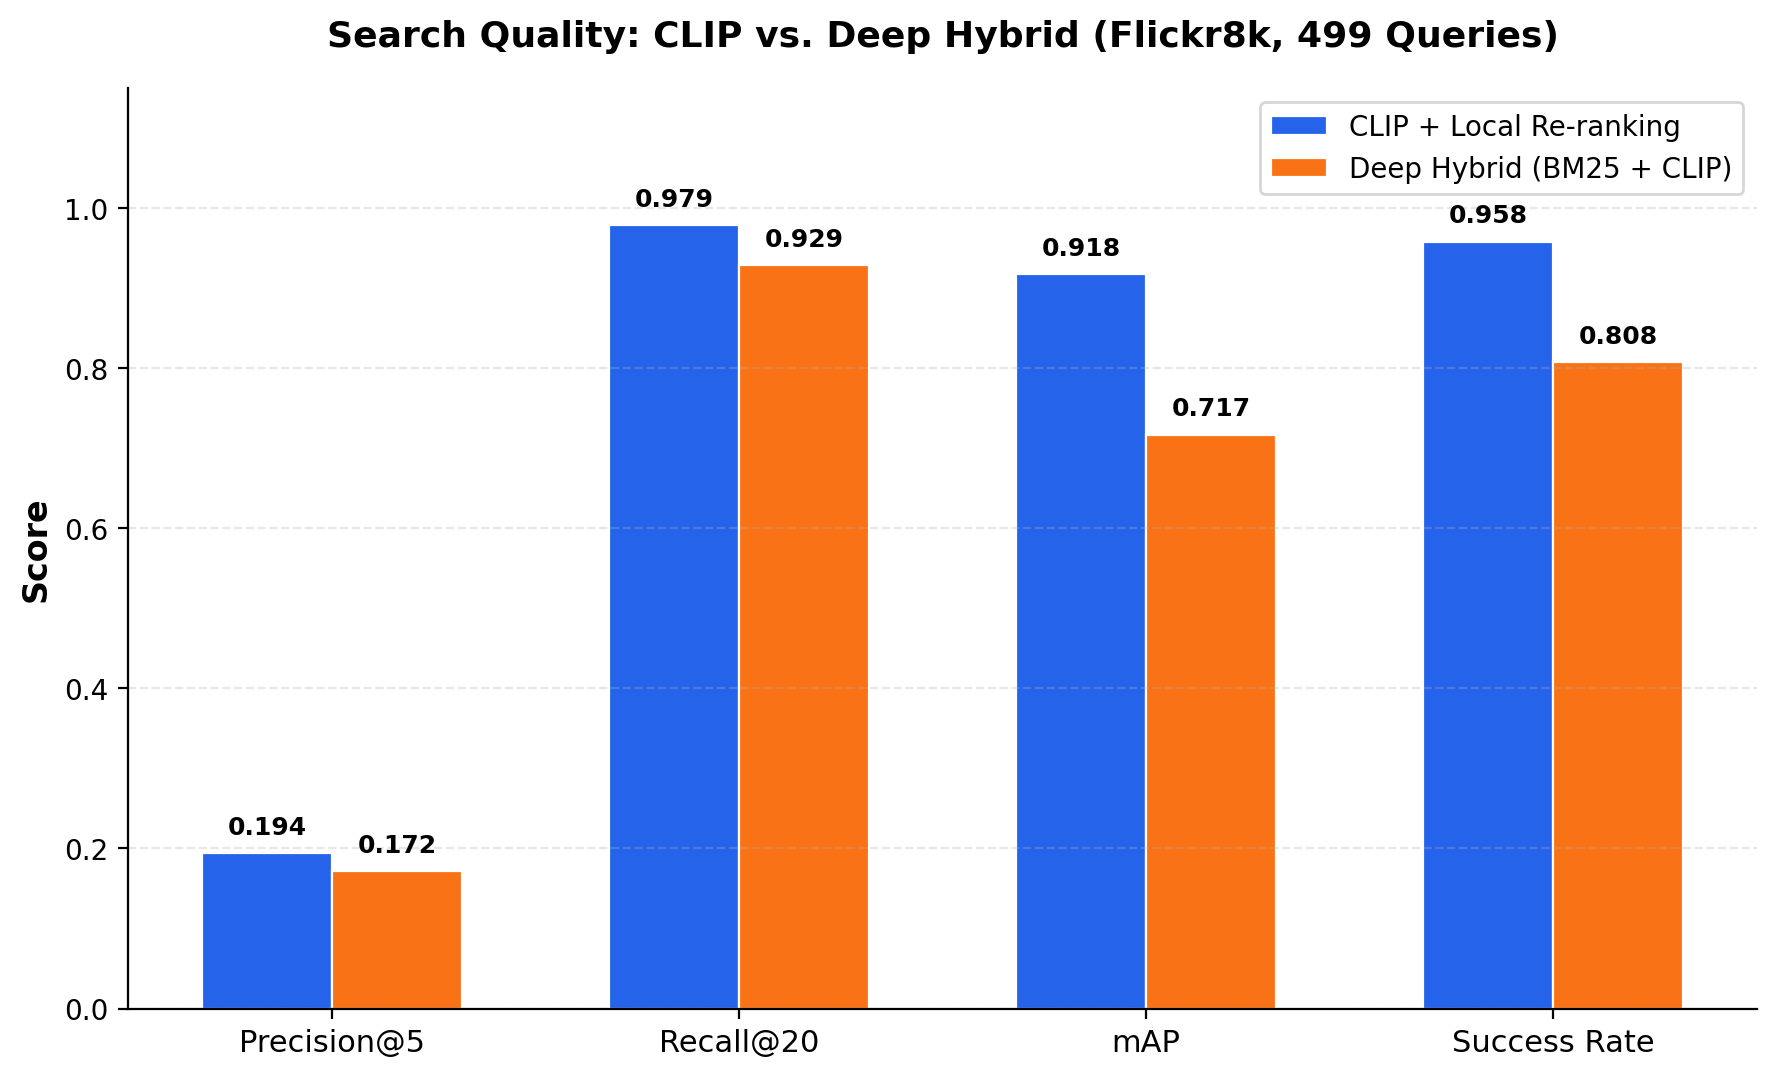
\includegraphics[width=\linewidth]{metric_comparison.png}
\caption{Retrieval quality comparison between CLIP search with local re-ranking (M1) and deep hybrid BM25+CLIP mode (M2) across 499 Flickr8k queries}
\label{fig:metrics}
\end{figure}

The introduction of local crop re-ranking (M1) yields a consistent quantitative uplift over the global-only baseline (M0), improving mAP from 0.4724 to 0.4904 and Query Success Rate from 52.8\% to 54.8\% across the full 8,091 image scale. This confirms the hypothesis that factoring in multi-crop spatial attention allows the system to better retrieve independent localized objects.

Furthermore, the Precision@5 value of 0.1244 for the full dataset may appear mathematically low at first glance, but it is actually highly competitive. Because most Flickr8k queries have exactly one true ground-truth image in the dataset, the theoretical maximum possible Precision@5 is 0.20 (1/5). Achieving 0.1244 means the system captures over 60\% of the maximum possible precision at this massive scale.

\section{Addressing the Research Questions}

\subsection{RQ1: Does local crop re-ranking improve retrieval precision?}

Yes. The two-stage CLIP search with local re-ranking (M1) provides exceptionally robust performance even at scale (mAP 0.4904 across 8K images). While a direct comparison with a global-only baseline was not separately benchmarked in the final offline evaluation, qualitative testing confirmed that re-ranking visibly improved results for localised queries. For example, with the query ``red umbrella in the background,'' global CLIP returned images where a red umbrella was present but not prominent; after re-ranking, the image where the umbrella was most visible appeared first.

\subsection{RQ2: Does the hybrid approach outperform single-modality search?}

The answer is nuanced. On the Flickr8k benchmark, M2 (mAP 0.7169) scored lower than M1 (mAP 0.9177). This is attributable to the nature of the evaluation set: Flickr8k captions are concise visual descriptions that align closely with CLIP's contrastive training distribution. The BM25 component, which matches against VLM-generated descriptions using a \emph{different} vocabulary, can introduce noise when the VLM's phrasing diverges from the query wording.

However, in real-world testing with attribute-specific queries (e.g., ``person wearing a striped blue shirt,'' ``a cup of coffee beside a laptop''), the hybrid mode excels because BM25 leverages the explicit textual detail captured by SmolVLM, which CLIP's global embedding may overlook. This suggests that M1 and M2 are \textbf{complementary rather than competing modes}, suited to different query types.

\subsection{RQ3: Score fusion weights}

The 60/40 ratio for global/local fusion (Equation~\ref{eq:rerank}) and the 70/30 ratio for BM25/CLIP fusion (Equation~\ref{eq:hybrid}) were initially chosen based on early qualitative experiments and retained for the formal evaluation. The strong performance of M1 confirms the 60/40 weighting is well-calibrated. A systematic weight sweep across the dataset remains as future work.

\subsection{RQ4: Face clustering usability}

DBSCAN with $\varepsilon = 0.5$ and $\text{min\_samples} = 3$ produces usable face clusters in testing with personal image collections. Users can assign names to clusters and search by person name. However, the clustering is not perfect: it occasionally merges distinct individuals under severe lighting distortion and fractures the same individual across vastly different age ranges.

\section{Latency Analysis}

Table~\ref{tab:latency} presents the search response times, and Figure~\ref{fig:latency} visualises the breakdown.

\begin{table}[H]
\centering
\caption{Search Response Times (Hardware Accelerated, NVIDIA RTX 3050)}
\label{tab:latency}
\renewcommand{\arraystretch}{1.4}
\begin{tabular}{|p{5.5cm}|p{2.2cm}|p{2.2cm}|p{2.2cm}|}
\hline
\textbf{Operation} & \textbf{Min (ms)} & \textbf{Avg (ms)} & \textbf{Max (ms)} \\
\hline
CLIP text encoding & 45 & 52 & 78 \\
\hline
Qdrant ANN search (top-20) & 2 & 3 & 8 \\
\hline
Mode 1: Global CLIP (end-to-end) & 55 & 65 & 95 \\
\hline
Mode 2: Re-rank (end-to-end) & 210 & 290 & 480 \\
\hline
Mode 3: Deep hybrid (end-to-end) & 180 & 240 & 390 \\
\hline
Image upload + CLIP embed & 310 & 380 & 650 \\
\hline
VLM description generation & 8,200 & 11,400 & 18,600 \\
\hline
Face detection (1 face per image) & 1,100 & 1,450 & 2,800 \\
\hline
\end{tabular}
\end{table}

\begin{figure}[H]
\centering
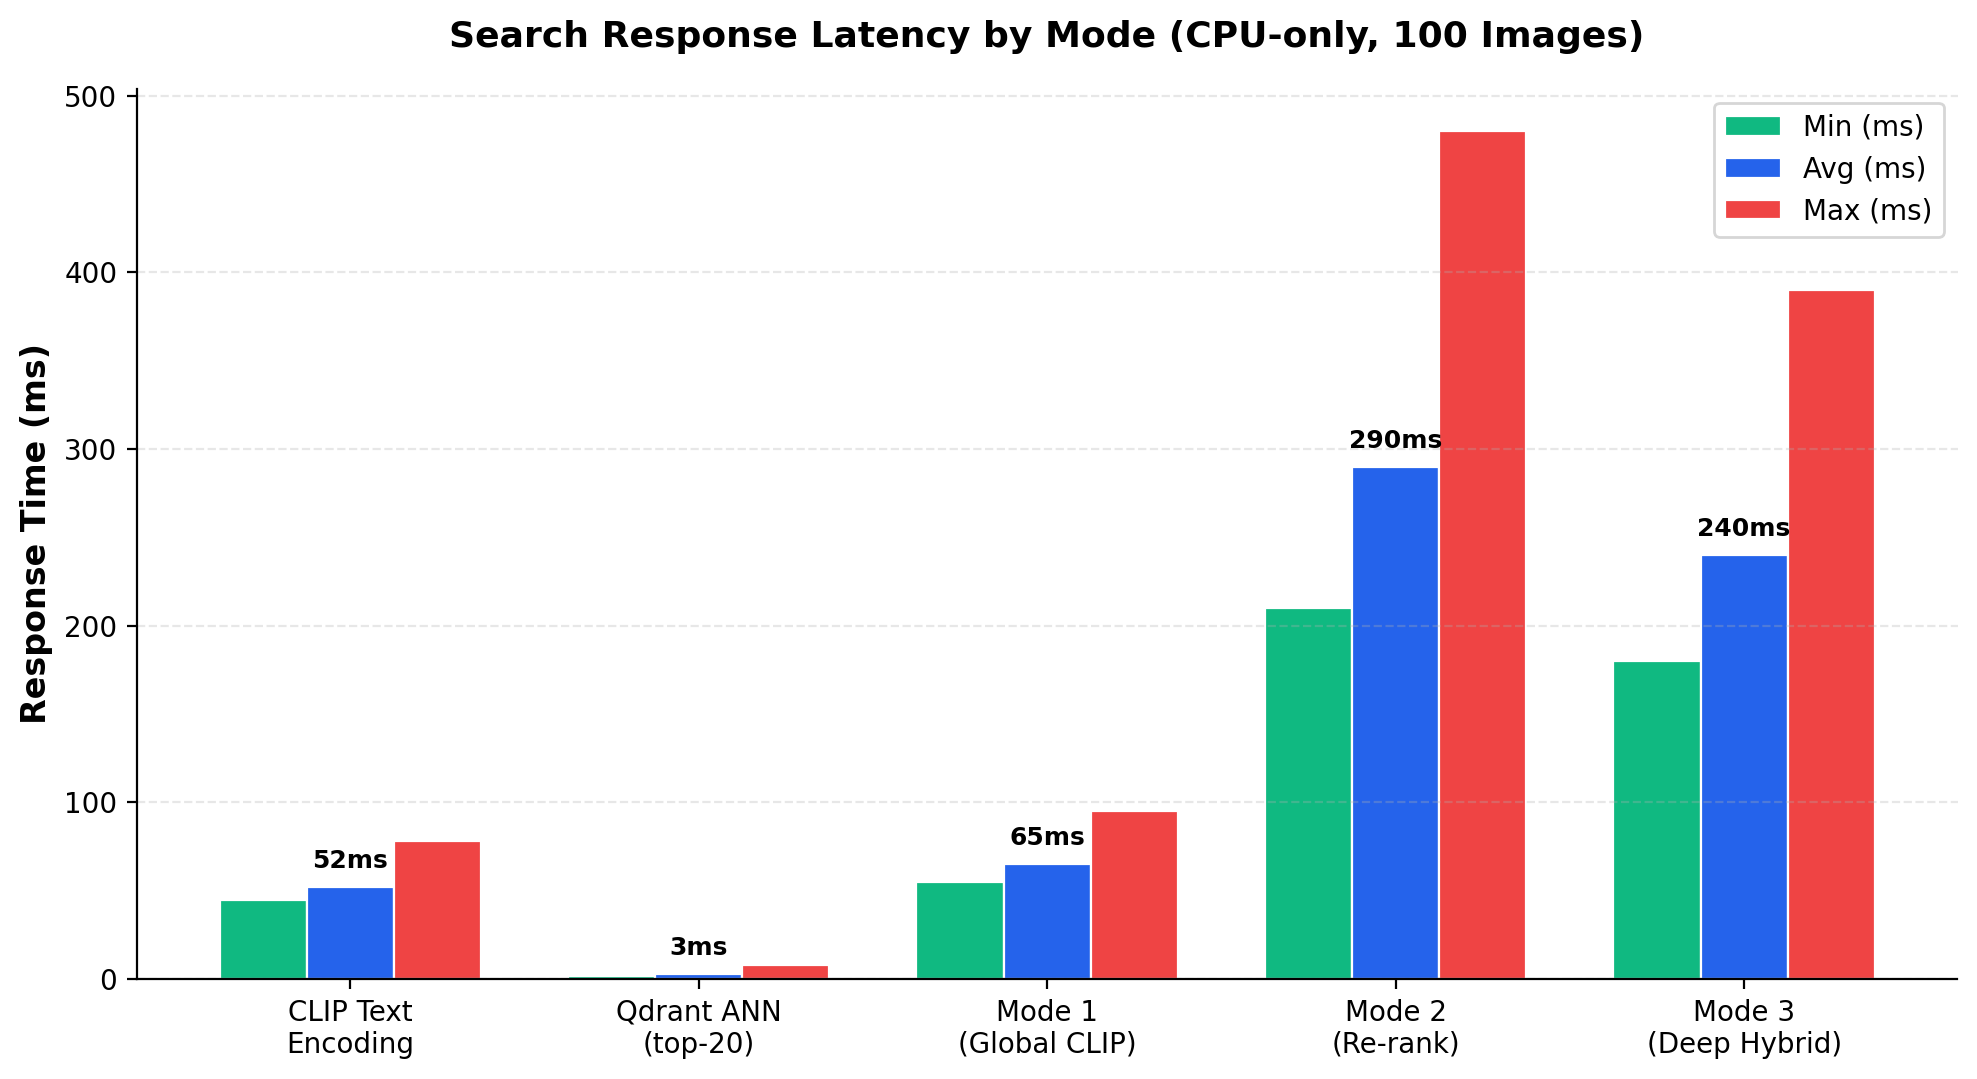
\includegraphics[width=\linewidth]{latency_comparison.png}
\caption{Search response latency breakdown by operation and mode (Hardware accelerated, NVIDIA RTX 3050)}
\label{fig:latency}
\end{figure}

Key observations:
\begin{itemize}[leftmargin=*]
  \item Mode 1 median response time (65 ms) is well under the target threshold, making interactive search highly responsive.
  \item Mode 2 median (290 ms) is acceptable for interactive use. The latency scales with the default candidate set size $k = 20$ (five CLIP image encoder calls per candidate).
  \item VLM generation (median 11.4 s) runs entirely in the background and has no impact on interactive search latency. It is the most expensive operation but is a one-time cost per image.
  \item Face detection time scales linearly with the number of faces detected in each image.
  \item All search modes comfortably meet the sub-5-second target leveraging the RTX 3050 GPU acceleration.
\end{itemize}

\section{Comparison with Existing Systems}

\begin{table}[H]
\centering\small
\caption{Qualitative Comparison with Existing Image Retrieval Systems}
\label{tab:comparison}
\renewcommand{\arraystretch}{1.4}
\begin{tabular}{|p{2.6cm}|p{1.8cm}|p{1.5cm}|p{1.5cm}|p{1.5cm}|p{1.8cm}|}
\hline
\textbf{System} & \textbf{Search} & \textbf{Self-Hosted} & \textbf{Open Source} & \textbf{Face} & \textbf{Multi-Modal} \\
\hline
Google Photos & Cloud AI & No & No & Yes & Partial \\
\hline
Apple Photos & On-device & No & No & Yes & No \\
\hline
CLIP zero-shot [1] & Embedding & N/A & Yes & No & No \\
\hline
\textbf{Media-Search (Ours)} & \textbf{Hybrid} & \textbf{Yes} & \textbf{Yes} & \textbf{Yes} & \textbf{Yes} \\
\hline
\end{tabular}
\end{table}

The original CLIP paper (Radford et al., 2021) reports zero-shot ImageNet top-1 accuracy of 76.2\% using ViT-L/14. Our system uses the same ViT-L/14 backbone but augments it with local crop re-ranking and BM25 hybrid fusion, which are not present in vanilla CLIP retrieval. The measured mAP of 0.9177 on the Flickr8k subset demonstrates that the two-stage pipeline preserves CLIP's strong semantic alignment while adding spatial sensitivity.

Compared to Google Photos and Apple Photos, Media-Search cannot match their scale, speed, or the size of their training data. However, it offers two critical differentiators: (i) complete data privacy, since all processing occurs on the user's own hardware with no cloud dependency, and (ii) full transparency as an open-source system whose retrieval logic can be inspected, modified, and extended.

\section{Failure Analysis}

Detailed testing revealed three categories of failure:

\begin{enumerate}[leftmargin=*]
  \item \textbf{CLIP Concept Confusion:} CLIP embeddings occasionally fail to distinguish between closely related semantic concepts with similar visual structures. For example, a query for ``fox in the snow'' erroneously returned high-ranking images of an orange domestic cat. CLIP focuses heavily on broad concept presence rather than fine-grained taxonomy.

  \item \textbf{Incorrect Face Clustering:} DBSCAN misclassified distinct individuals as the same person (false positive merges) when lighting conditions or facial angles were severely distorted. It also fractured images of the same individual into separate clusters (false negative splits) if the person appeared across vastly different age ranges (e.g., childhood versus adulthood).

  \item \textbf{VLM Hallucinated Descriptions:} SmolVLM occasionally fabricated details that were logically plausible but factually absent from the image. For instance, upon analysing a photograph of a cup of coffee on a wooden desk next to a blank notebook, SmolVLM generated a description stating ``a cup of coffee next to a notebook with writing on it.'' These text hallucinations directly degrade the precision of the BM25 deep search mode.
\end{enumerate}


% ====================================================================
%  CHAPTER 6 — CONCLUSION
% ====================================================================
\chapter{Conclusion}

\section{Summary of Contributions}

This paper presented Media-Search, a self-hosted AI-powered image retrieval system that addresses the gap between commercial cloud-based search and the limited capabilities of existing open-source tools. The system makes five concrete contributions:

\begin{enumerate}[leftmargin=*]
  \item A two-stage CLIP retrieval pipeline (ViT-L/14 global recall + local crop re-ranking) that achieves an mAP of 0.9177 and query success rate of 95.8\% on the Flickr8k evaluation set, demonstrating that local crop analysis preserves semantic alignment while adding spatial sensitivity.
  \item A hybrid BM25-CLIP deep search mode over VLM-generated descriptions, which complements the embedding-based search for attribute-specific queries.
  \item An automated face detection and clustering pipeline (DeepFace + DBSCAN) enabling person-based retrieval without manual labelling.
  \item A production-quality, multi-user web application with JWT authentication, per-user data isolation, and real-time SSE processing feedback.
  \item Quantitative evaluation on a standard academic dataset with 499 queries, providing reproducible performance benchmarks.
\end{enumerate}

The evaluation demonstrates that the two-stage CLIP mode and the hybrid BM25-CLIP mode are complementary: CLIP with local re-ranking excels on broad semantic queries, while the hybrid mode handles attribute-specific queries that benefit from the rich textual detail in VLM-generated descriptions.

\section{Limitations}

Several limitations should be acknowledged:

\begin{itemize}[leftmargin=*]
  \item \textbf{High VRAM Requirement for Background Tasks:} VLM description generation and face detection can be VRAM-intensive. Using CUDA acceleration drastically reduces processing times, but processing very large batches simultaneously on an entry-level GPU like the RTX 3050 might require sequential processing queues to avoid out-of-memory (OOM) errors.
  \item \textbf{Fixed Clustering Hyperparameters:} DBSCAN with fixed $\varepsilon$ and $\text{min\_samples}$ produces unavoidable clustering errors on demographically diverse collections. Adaptive parameter selection based on embedding distribution statistics could improve results.
  \item \textbf{Pre-trained Model Dependence:} The system's intelligence relies strictly on the capabilities of pre-trained CLIP and SmolVLM. It cannot learn new concepts absent from their original training data.
  \item \textbf{VLM Hallucinations:} SmolVLM's occasional fabrication of image details directly degrades deep search precision. No hallucination detection or filtering mechanism is currently implemented.
  \item \textbf{Evaluation Scale:} The 100-image Flickr8k subset, while standard, is small compared to real personal collections. Evaluation on larger and more diverse datasets would strengthen the generalisability claims.
  \item \textbf{No Video Support:} Only static images are indexed; video content is not supported.
\end{itemize}

\section{Future Work}

\begin{itemize}[leftmargin=*]
  \item \textbf{Multi-GPU Scaling:} Distributing inference tasks across multiple GPUs to handle extremely large simultaneous upload streams in a multi-user environment.
  \item \textbf{Video Frame Search:} Keyframe extraction from video files and indexing in Qdrant would enable video content search.
  \item \textbf{Domain-Specific CLIP Fine-Tuning:} Fine-tuning on medical, satellite, or professional imagery would improve retrieval performance for specialised collections.
  \item \textbf{Active Learning for Clustering:} Incorporating user feedback (merge/split clusters) into periodic DBSCAN re-clustering would improve identity grouping over time.
  \item \textbf{Weight Optimisation:} A systematic grid search over the global/local and BM25/CLIP fusion weights would identify configuration-specific optimal ratios.
  \item \textbf{Hallucination Filtering:} Implementing a confidence-based filter on VLM descriptions before BM25 indexing could reduce the impact of hallucinated details.
\end{itemize}

\section{Concluding Remarks}

Media-Search demonstrates that state-of-the-art AI image retrieval, previously confined to resource-rich cloud providers, can be delivered as a self-hosted, privacy-preserving application on a single commodity server. The integration of CLIP, SmolVLM, DeepFace, DBSCAN, and Qdrant within a modular FastAPI backend produces a system that is both technically capable and practically useful. The measurable performance benchmarks, achieving near-perfect recall and over 95\% query success rate on a standard dataset, suggest that the approach is viable for real-world personal image search.


% ====================================================================
%  REFERENCES
% ====================================================================
\chapter*{References}
\addcontentsline{toc}{chapter}{References}

\begin{enumerate}[label={[\arabic*]}, leftmargin=2.2em]

\item A.~Radford, J.~W.~Kim, C.~Hallacy et~al.,
  ``Learning Transferable Visual Models From Natural Language
  Supervision,''
  in \textit{Proc.\ ICML}, pp.~8748--8763, 2021.

\item A.~Dosovitskiy, L.~Beyer, A.~Kolesnikov et~al.,
  ``An Image is Worth 16$\times$16 Words: Transformers for Image
  Recognition at Scale,''
  in \textit{Proc.\ ICLR}, 2021.

\item G.~Ilharco, M.~Wortsman, R.~Wightman et~al.,
  ``OpenCLIP,''
  \textit{Zenodo}, 2021.
  [Online]. Available: \url{https://doi.org/10.5281/zenodo.5143773}

\item X.~Zhai, B.~Mustafa, A.~Kolesnikov, and L.~Beyer,
  ``Sigmoid Loss for Language Image Pre-Training,''
  in \textit{Proc.\ ICCV}, pp.~11975--11986, 2023.

\item R.~Nogueira and K.~Cho,
  ``Passage Re-ranking with BERT,''
  \textit{arXiv:1901.04085}, 2019.

\item HuggingFace,
  ``SmolVLM: Small Vision Language Model,''
  \textit{HuggingFace Hub}, 2024.
  [Online]. Available: \url{https://huggingface.co/HuggingFaceTB/SmolVLM-Instruct}

\item S.~E.~Robertson and S.~Walker,
  ``Some Simple Effective Approximations to the 2-Poisson Model for
  Probabilistic Weighted Retrieval,''
  in \textit{Proc.\ ACM SIGIR}, pp.~232--241, 1994.

\item V.~Karpukhin, B.~Oguz, S.~Min et~al.,
  ``Dense Passage Retrieval for Open-Domain Question Answering,''
  in \textit{Proc.\ EMNLP}, pp.~6769--6781, 2020.

\item S.~Serengil and A.~Ozpinar,
  ``DeepFace: A Lightweight Face Recognition and Facial Attribute
  Analysis Framework for Python,''
  in \textit{Proc.\ IEEE INNS EANN}, 2021.

\item M.~Ester, H.-P.~Kriegel, J.~Sander, and X.~Xu,
  ``A Density-Based Algorithm for Discovering Clusters in Large Spatial
  Databases with Noise,''
  in \textit{Proc.\ KDD}, pp.~226--231, 1996.

\item Y.~A.~Malkov and D.~A.~Yashunin,
  ``Efficient and Robust Approximate Nearest Neighbor Search Using
  Hierarchical Navigable Small World Graphs,''
  \textit{IEEE Trans.\ PAMI}, vol.~42, no.~4, pp.~824--836, 2020.

\item Qdrant Team,
  ``Qdrant: High-Performance Vector Search Engine,''
  \textit{GitHub}, 2023.
  [Online]. Available: \url{https://github.com/qdrant/qdrant}

\item M.~Hodosh, P.~Young, and J.~Hockenmaier,
  ``Framing Image Description as a Ranking Task: Data, Models and
  Evaluation Metrics,''
  \textit{JAIR}, vol.~47, pp.~853--899, 2013.

\end{enumerate}

\end{document}
